\documentclass[11pt]{article}\usepackage{graphicx, color}
%% maxwidth is the original width if it is less than linewidth
%% otherwise use linewidth (to make sure the graphics do not exceed the margin)
\makeatletter
\def\maxwidth{ %
  \ifdim\Gin@nat@width>\linewidth
    \linewidth
  \else
    \Gin@nat@width
  \fi
}
\makeatother

\IfFileExists{upquote.sty}{\usepackage{upquote}}{}
\definecolor{fgcolor}{rgb}{0.2, 0.2, 0.2}
\newcommand{\hlnumber}[1]{\textcolor[rgb]{0,0,0}{#1}}%
\newcommand{\hlfunctioncall}[1]{\textcolor[rgb]{0.501960784313725,0,0.329411764705882}{\textbf{#1}}}%
\newcommand{\hlstring}[1]{\textcolor[rgb]{0.6,0.6,1}{#1}}%
\newcommand{\hlkeyword}[1]{\textcolor[rgb]{0,0,0}{\textbf{#1}}}%
\newcommand{\hlargument}[1]{\textcolor[rgb]{0.690196078431373,0.250980392156863,0.0196078431372549}{#1}}%
\newcommand{\hlcomment}[1]{\textcolor[rgb]{0.180392156862745,0.6,0.341176470588235}{#1}}%
\newcommand{\hlroxygencomment}[1]{\textcolor[rgb]{0.43921568627451,0.47843137254902,0.701960784313725}{#1}}%
\newcommand{\hlformalargs}[1]{\textcolor[rgb]{0.690196078431373,0.250980392156863,0.0196078431372549}{#1}}%
\newcommand{\hleqformalargs}[1]{\textcolor[rgb]{0.690196078431373,0.250980392156863,0.0196078431372549}{#1}}%
\newcommand{\hlassignement}[1]{\textcolor[rgb]{0,0,0}{\textbf{#1}}}%
\newcommand{\hlpackage}[1]{\textcolor[rgb]{0.588235294117647,0.709803921568627,0.145098039215686}{#1}}%
\newcommand{\hlslot}[1]{\textit{#1}}%
\newcommand{\hlsymbol}[1]{\textcolor[rgb]{0,0,0}{#1}}%
\newcommand{\hlprompt}[1]{\textcolor[rgb]{0.2,0.2,0.2}{#1}}%

\usepackage{framed}
\makeatletter
\newenvironment{kframe}{%
 \def\at@end@of@kframe{}%
 \ifinner\ifhmode%
  \def\at@end@of@kframe{\end{minipage}}%
  \begin{minipage}{\columnwidth}%
 \fi\fi%
 \def\FrameCommand##1{\hskip\@totalleftmargin \hskip-\fboxsep
 \colorbox{shadecolor}{##1}\hskip-\fboxsep
     % There is no \\@totalrightmargin, so:
     \hskip-\linewidth \hskip-\@totalleftmargin \hskip\columnwidth}%
 \MakeFramed {\advance\hsize-\width
   \@totalleftmargin\z@ \linewidth\hsize
   \@setminipage}}%
 {\par\unskip\endMakeFramed%
 \at@end@of@kframe}
\makeatother

\definecolor{shadecolor}{rgb}{.97, .97, .97}
\definecolor{messagecolor}{rgb}{0, 0, 0}
\definecolor{warningcolor}{rgb}{1, 0, 1}
\definecolor{errorcolor}{rgb}{1, 0, 0}
\newenvironment{knitrout}{}{} % an empty environment to be redefined in TeX

\usepackage{alltt}

%AMS-TeX packages
\usepackage{amssymb,amsmath,amsthm} 
%geometry (sets margin) and other useful packages
\usepackage[margin=1in]{geometry}
\usepackage{graphicx, ctable, booktabs}
\usepackage{color}
\usepackage{listings}
\usepackage{ltablex, calc, enumerate, multirow, float, soul}
\usepackage{hyperref}
\usepackage{longtable, pdflscape, textcase}

\begin{document}



\setlength{\parskip}{3ex}
\setlength{\parindent}{0pt}

\title{Can you buy a president? \\ \vspace{.6cm} \Large Politics after the Tillman Act}
\author{Eric Hare \& Andee Kaplan}
\date{Dec. ??, 2012}

\maketitle
\thispagestyle{empty}
\begin{abstract}
Motivated by the 2010 Citizens United ruling and the subsequent birth of ``Super PACs", this paper uses independent expenditures data from the Federal Elections Commission, in conjunction with presidential polling data to analyze the 2012 presidential campaign. Using R, and the packages \texttt{XML}, \texttt{ggplot2}, \texttt{plyr}, \texttt{lubridate}, \texttt{knitr}, \texttt{forecast}, and \texttt{zoo}, we scrape data from these sources and analyze them in order to highlight interesting trends in campaign spending. Furthermore, we correlate these trends in spending over time to the changes in the polls. Ultimately, we did not find a clear and direct relationship between increases in spending and changes in public support. However, our analysis does provide evidence for some commonly held views of the candidate's spending habits and geographical areas of strength and weakness.
\end{abstract}
\clearpage

\setcounter{page}{1}
\section{Introduction}
A Political Action Committee (PAC) is defined as any organization that seeks to influence the outcome of an election or policy decision through financial donations. Until recently, there have been strict regulations in place limiting the amount of money that individuals and corporations could donate to PACs.

In 2010, the United States Supreme Court released its decision on Citizens United v. Federal Election Commission. The decision found that it is a violation of the constitutional right to free speech for limits to be placed on money spent by corporations and labor unions to support or oppose political candidates. For the first time since the passage of the Tillman Act in 1907, corporations and unions could spend unlimited amounts of their own money on the presidential election. Such power led to the coining of the term Super PAC, as well as a cloud of uncertainty as to what effect such money could have on the election outcome. Three of the largest Super PACs, American Crossroads, Restore our Future, and Priorities USA Action, spent over \$305M in the 2012 election cycle alone. In 2008, PACs spent over \$151M on the presidential election (not including primaries), or approximately \$0.50 per US citizen. In 2012, PACs and Super PACs spent over \$560M, or approximately \$1.78 per US citizen. With this 350\% increase in spending the fear is that a group of individuals or corporations can buy a president.


In this report, we analyze independent expenditures filings from the Federal Election Commission in an attempt to determine the effect of this spending on the 2012 election.  We subset these expenditures to analyze only those which were filed after the Republican primary, so that we can focus on those which benefit President Barack Obama and Governor Mitt Romney. We also retrieve data from the NationalPolls.com database of polling results to quantify the effect of this spending. The results of our analysis suggest that the spending may have had a measurable impact on public opinion, but external factors, such as the presidential debates, had much stronger impacts.






\section{Data}
We are primarily working with two data sources to complete our analysis: independent expenditures (PAC) data and polling data. The \href{http://www.fec.gov/data/IndependentExpenditure.do?format=html&cf=superPAC}{Federal Election Commission} keeps track of the PAC spending filings and makes the information publicly available. The polling data comes from \href{http://nationalpolls.com/}{NationalPolls.com}, a website which aggregates national and state polls from multiple polling companies. We are primarily working with the fields spe\_nam, exp\_amo, exp\_dat, and pur from the spending data. These provide us with information on the organization filing the expense, the amount, the date, and the purpose of the expense. We also make extensive use of our created field, beneful\_can, which indicated which candidate benefitted from the expense. A description of the fields used most in the spending data set is provided in Table \ref{tab:spendData} and a decription of the fields used in the polling data set is provided in Table \ref{tab:pollData}. A full descripton of all fields available from the FEC and NationalPolls.com is available in our supplementary materials.

\begin{table}[h!]
\begin{tabular}[\textwidth]{l l p{0.55\textwidth}}
Tag & Field Name & Description  \\
\hline
\hline
\multicolumn{3}{l}{\MakeTextUppercase{Character Variables}}\\
\hline
%can\_id  & Candidate ID & Unique ID of candidate for or against whom the expenditure was made. First character indicates office sought - H=House, S=Senate, P=Presidential. Columns 3-4 are the state abbreviation for Congressional candidates. NOTE - this information is provided by filers and may be missing - in these cases office, state, district and candidate name should appear.\\
can\_nam & Candidate Name & Name of candidate for or against whom the expenditure was made. There are 58 unique presidential candidate names in the data set, but they do not identify candidates uniquely. For example, there are eight unique spellings of Mr. Obama's name.\\
%spe\_id & Spender ID & Unique ID of committee, individual or group making expenditure. Unique FEC ID assigned to the entity submitting reports of independent expenditures.\\
spe\_nam & Spender Name &	Name of committee, individual or group making expenditure.\\
%ele\_typ & Election Type & Code for specific election for which expenditure was made. First character indicates election - P=Primary, G=General, S=Special. Next four characters indicate election year.\\
%can\_off\_sta & Candidate State	& Postal state abbreviation for the candidate.\\
can\_off & Office &	Office Sought by Candidate - H=House, S=Senate, P=President.\\
%can\_par\_aff &	Party &	Party abbreviation for candidate - Dem=Democrat, Rep=Republican.\\
sup\_opp &  Support or Oppose &	Describes whether the expenditure was made to support or oppose the candidate - S=Support, O=Oppose.\\	 
pur &	Purpose of expenditure &	Description of the expenditure, e.g. television or radio ad.\\
pay &	name of payee &	Name of the person or vendor or other entity receiving this payment.\\
%amn\_ind &  Amendment Indicator &	New report or amendment to a report	& \\	 
%tra\_id	& Transaction ID & Unique identifier for the transaction (unique within the specific filing.\\
\hline
\multicolumn{3}{l}{\MakeTextUppercase{Currency Variables}}\\
\hline
exp\_amo & Expenditure Amount & Dollar amount of specific expenditure. \newline 
Min: \$0 \newline
Max: \$17,661,251 \newline
Mean: \$11,306.42 \newline
Median: \$26.61\\
%agg\_amo & Aggregate amount &	Total amount expended during the calendar year, per election, per office sought. \newline 
%Min: \$format(min(spend.data$agg_amo, na.rm=TRUE), nsmall=2, scientific=FALSE) \newline
%Max: \$format(max(spend.data$agg_amo, na.rm=TRUE), nsmall=2, scientific=FALSE) \newline
%Mean: \$format(mean(spend.data$agg_amo, na.rm=TRUE), nsmall=2, scientific=FALSE) \newline
%Median: \$format(median(spend.data$agg_amo, na.rm=TRUE), nsmall=2, scientific=FALSE)\\
\hline
\multicolumn{3}{l}{\MakeTextUppercase{Date Variables}}\\
\hline
exp\_dat &  Expenditure date & Date of specific Expenditure	MM/DD/YYYY.\\
%rec\_dt  & Filing receipt date & Date on which transaction was submitted to FEC	MM/DD/YYYY.\\
%\hline
%\multicolumn{3}{l}{\MakeTextUppercase{Numeric Variables}}\\
%\hline
%can\_off\_dis &  Candidate District &	District number for the candidate. District location if spending for/against House candidate.\\
%file\_num  & Filing number &	Unique identifier for a submission (which may report several disbursements).\\
%ima\_num &	Image number &	Image location for page on which transaction appears.\\	 
%prev\_file\_num & Previous filing number &	Reference to a filing being amended. For electronic filings the previous filing number references the filing being amended. For new filings and paper filings this field will be null.
\hline
\multicolumn{3}{l}{\MakeTextUppercase{Derived Variables}}\\
\hline
bucket & Category of expenditure & Low level categories detailing what the expenditure was for. Examples include television, internet, and radio ads.\\
bucket2 & High level category & High level categories detailing what the expenditure was for. Examples include ads, transport, and swag.\\
oflag & Obama flag & Flag indicating if this record is associated with Obama or Romney - 1 = Obama, 0 = Romney.\\
beneful\_can & Benefitting candidate & Name of candidate that benefits from the expenditure. For example, a record with \texttt{sup\_opp} = ``oppose" and \texttt{can\_nam} = ``Romney" will benefit Mr. Obama.\\
\end{tabular}
\caption{Description of spending data fields.}
\label{tab:spendData}
\end{table}

\begin{table}[h!]
\begin{tabular}{l p{0.4\textwidth} p{0.45\textwidth}}
Tag & Field Name & Description\\
\hline
\hline
\multicolumn{3}{l}{\MakeTextUppercase{Character Variables}}\\
\hline
Pollster & Polling Company & Company that conducted the poll. \\
State/US & State & State poll was conducted of. If national poll, then value is ``National".\\
\hline
\multicolumn{3}{l}{\MakeTextUppercase{Date Variables}}\\
\hline
Date & Poll Date & Range of dates that the poll was being conducted.\\
\hline
\multicolumn{3}{l}{\MakeTextUppercase{Numeric Variables}}\\
\hline
Obama & Support for Mr. Obama & Integer rounded percent of support in the poll. \\
Romney & Support for Mr. Romney & Integer rounded percent of support in the poll.
\end{tabular}
\caption{Description of polling data fields.}
\label{tab:pollData}
\end{table}

We spent a significant amount of time cleaning the the PAC spending data in order to make it usable for our analysis. We used pattern recognition as well as text manipulation methods to accomplish the cleaning. Even seemingly simple analyses like counting the number of expenditures benefitting each candidate were made more complicated by the reality of the data. Complications arose from multiple issues, the first being the lack of standardization in the can\_nam field. For example, Mr. Obama's name was spelled eight different ways and Mr. Romney's name was spelled seven different ways. See Table \ref{tab:can_nam} for details. 


% latex table generated in R 2.15.2 by xtable 1.7-0 package
% Thu Jan 10 19:02:19 2013
\begin{table}[ht]
\begin{center}
\begin{tabular}{rll}
  \hline
 & Mr.Obama & Mr.Romney \\ 
  \hline
1 & obama, barack & romney, mitt / ryan, paul d. \\ 
  2 & barack, obama & romney, w mitt \\ 
  3 & obama, barak & romney, mitt \\ 
  4 & barak, obama & mitt, romney \\ 
  5 & obama, barack hussein & romney / paul d. ryan, mitt \\ 
  6 & obama, barak hussein & romney, mary rose \\ 
  7 & 2012, obama/biden & romney, willard \\ 
  8 & obama, pres. barack &  \\ 
   \hline
\end{tabular}
\caption{Multiple spellings of candidate names in spending data.}
\label{tab:can_nam}
\end{center}
\end{table}




An additional complication we faced was with the support/oppose column (\texttt{sup\_opp}). This column in conjunction with the candidate column are used to indicate which candidate benefits from the expenditure. An example would be if the support/oppose value is ``oppose'' and the candidate name is ``Romney'', then Mr. Obama benefits because the money is being spent to ``oppose Romney". Likewise, if the support/oppose column equals ``support'' and the candidate name is ``Romney'', then Mr. Romney benefits.  We solved this by adding a new field which simply stores the candidate that benefits from the particular expense.  That is, an opposition advertisement expense entered with a candidate name of Obama will benefit Romney. However, 15 Super PACs appeared to support both candidates (see Table \ref{tab:prob_spe}). After researching these PACs, we found that they were not in fact bipartisan supporters, and concluded that an entry error had been made on those filings. We coded those records to indicate support of the candidate most often benefitted by those PACs.


% latex table generated in R 2.15.2 by xtable 1.7-0 package
% Thu Jan 10 19:02:19 2013
\begin{table}[ht]
\begin{center}
\begin{tabular}{rl}
  \hline
 & PAC.Names \\ 
  \hline
1 & 1199seiu united healthcare workers east \\ 
  2 & america vs obama \\ 
  3 & american federation of state county and municipal employees afl-cio \\ 
  4 & campaign to defeat barack obama \\ 
  5 & house majority pac \\ 
  6 & jewish council for education and research \\ 
  7 & lcv victory fund \\ 
  8 & liberty action pac \\ 
  9 & naral pro-choice america \\ 
  10 & national rifle association institute for legislative action \\ 
  11 & service employees international union pea - federal \\ 
  12 & unite here tip state \& local fund \\ 
  13 & voces de la frontera action \\ 
  14 & workers' voice \\ 
  15 & working america \\ 
   \hline
\end{tabular}
\caption{Super PACs appearing to support both candidates.}
\label{tab:prob_spe}
\end{center}
\end{table}




Another serious challenge we faced was that the purpose of independent expenditures column is a free text field on the FEC reporting form with 1,466 unique entries. For example, the conservative Super PAC Americans for Prosperity tended to use verbose descriptions of the spending purpose. An entry from mid-August read ``oppose advertising-tv production (voted for)." This description lists whether it was an ad in support or opposition, that it was a television ad, and the name of the ad. In contrast, the anti-abortion Women Speak Out PAC preferred short descriptions, such as ``ads" for their early-October expense. The result was that when trying to explore what PACs spent the majority of their money on, we were unable to group expenditures together. To solve this issue we searched for matches to patterns in the purpose field. We chose these patterns by looking at the expenditure purposes and manually finding common threads among the purposes. From these patterns we were able to create buckets that each expense fell in to, as well as high level buckets that more generally classified the expenditures. The buckets we chose are: 

\begin{description}
    \item[Ads] Advertisement spending, including television, radio, and online
    \item[Direct Contact] Direct voter contact, such as canvassing
    \item[Salary] Payments made to staff of the organization
    \item[Swag] Clothing, signs, and other promotional material
    \item[Transport] Transportation costs, such as taxis or van rentals
    \item[Other] All expenses that do not fit into the above categories
\end{description}

Both of the example records above (the Americans for Properity and Women Speak Out PAC expenditures) have a high-level classification (bucket\_2) of ``ad", while they have a low-level classification (bucket) of ``tv" and ``media", respectively.

The polling data did not require much data cleanup. We split the date range and formatted the end date as a date for our use. We also removed some differences in state naming by the different pollsters.  One limitation we faced is that a fairly significant number of polls were excluded from the NationalPolls.com database.  Some new national polling outfits, such as the RAND Corporation, were excluded, as were a large number of online polls, including Google Consumer Surveys.  Online surveys performed more strongly in the 2012 election than did automated phone surveys or live interviewer surveys according to New York Times columnist Nate Silver \footnote{\href{http://fivethirtyeight.blogs.nytimes.com/2012/11/10/which-polls-fared-best-and-worst-in-the-2012-presidential-race/}{Which Polls Fared Best (and Worst) in the 2012 Presidential Race}}.  Polling aggregators may want to examine the performance of new survey techniques more closely and consider including them in future elections.


\section{Findings}
Our key findings are summarized in the following sections.  We begin by analyzing the spending patterns of Super PACs over the duration of the election season. We then take a closer look at the organizations which are spending the most on each side. Next, we analyze changes in the polling data with an emphasis on swing states. We conclude by attempting to correlate these changes to spending changes over time.

%\subsection{Type of Spending by Week}
Although a cursory look at the data suggests large and frequent spending benefitting both candidates, we set out to explore how this spending changed over time.  Futhermore, we wanted see whether Super PACs benefitting Mr. Obama tended to allocate resources to different buckets when compared to Super PACs benefitting Mr. Romney.  Such differences, if they were to exist, may help future successful campaigns distribute their resources more effectively. Figure \ref{fig:temporal_plot} displays the spending in each of the six categories by independent organizations benefiting Mr. Obama and Mr. Romney for each week since April 25, 2012. The spending amounts are split by whether the goal was to support or oppose the candidate. There are three markers which signify major events in the campaign: the selection of Representative Paul Ryan as Mr. Romney's vice presidential nominee, the Republican National Convention, the Democratic National Convention, the 47\% video, and the debates.

Interesting trends can be observed in advertisement spending, and direct contact. Ads in support of both candidates show increases since the end of July. However, ads in opposition of the candidates were airing well before. You can, however, see an increase in negative ads benefiting Mr. Romney. A noticeable increase in spending on direct contact for Obama is also evident beginning in August, while the organizations benefiting Mr. Romney have maintained consistent spending in negative direct contact beginning in mid-May.  Furthermore, ad spending in both support and opposition by Super PACs benefitting Mr. Romney was a factor of $10^5$ higher than those by Super PACs benefitting Mr. Obama since the end of July.

Two of the advertisement weekly spending totals are highlighted in green.  These points mark extremely sharp increases in spending for Super PACs benefitting Mr. Romney.

\begin{knitrout}
\definecolor{shadecolor}{rgb}{0.969, 0.969, 0.969}\color{fgcolor}\begin{figure}[H]


{\centering 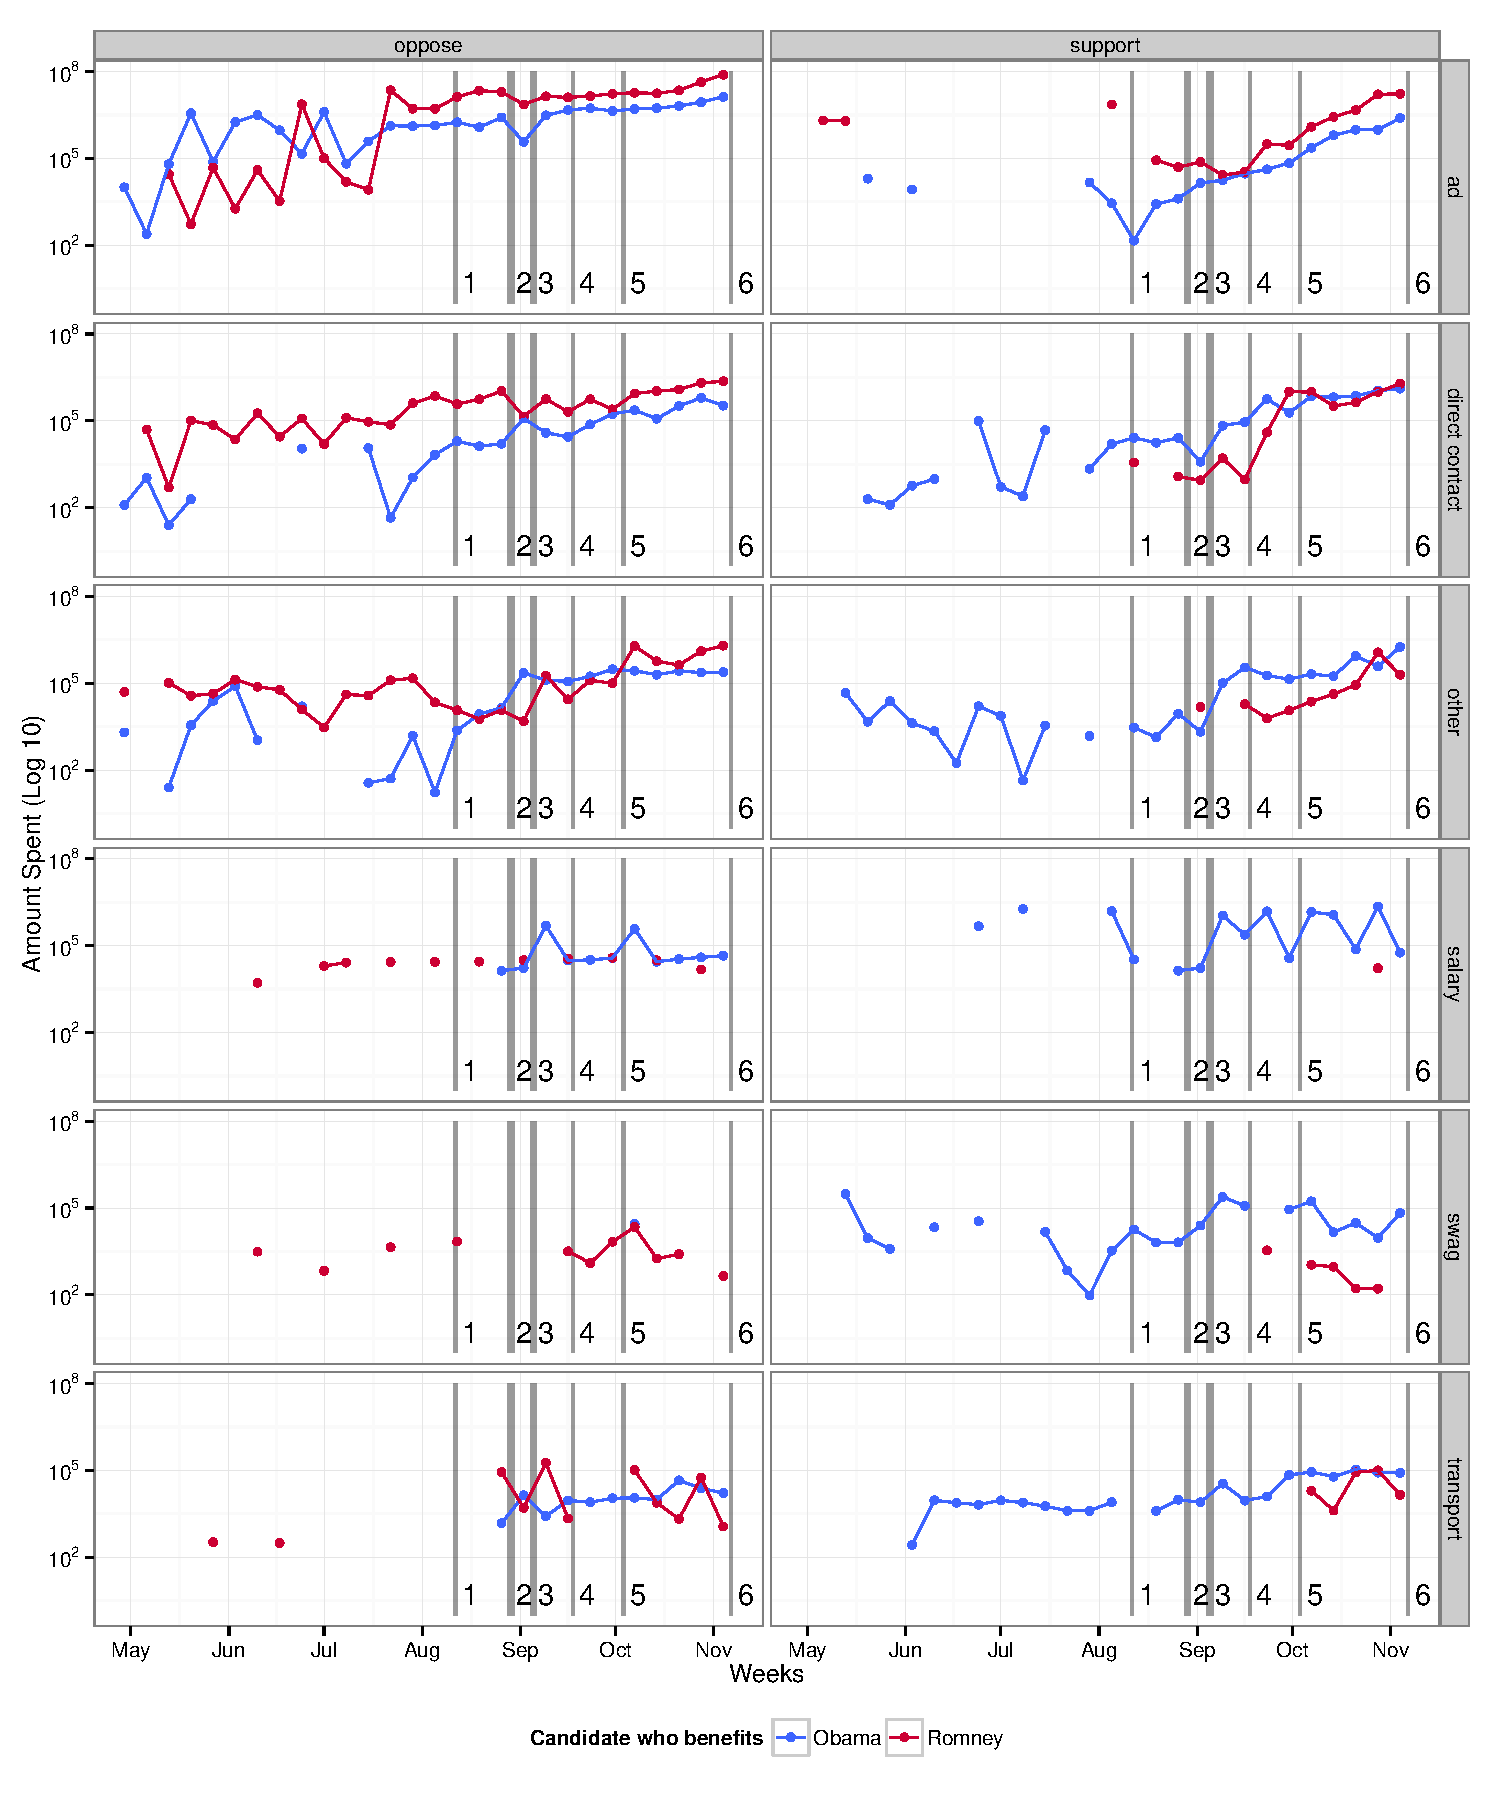
\includegraphics[width=\textwidth]{figure/temporal_plot} 

}

\caption[Total weekly spending by Super PACs in support or opposition of candidates]{Total weekly spending by Super PACs in support or opposition of candidates. Important events are indicated as follows: (1) Paul Ryan VP selection, (2) Republican National Convention, (3) Democratic National Convention, (4) 47\% video leaked, (5) first presidential debate, and (6) election day.\label{fig:temporal_plot}}
\end{figure}

\end{knitrout}



%\subsection{Spending Categories}
% The plots in Figure \ref{fig:type_plot} show the comparison of amount spent for each candidate by categories of independent expenditure, since April 25, 2012. The categories are mined from the self-reported text description of the expense. The left plot shows the spending to benefit Mr. Obama against the spending to benefit Mr. Romney by category, with values to the right of the reflection line showing PACs supporting Mr. Romney are outspending PACs supporting Mr. Obama on these categories, and vice verse for those to the left. The right plot shows bar chart comparisons of the spending in main categories, on a log scale.
% %, and bar charts showing overall spending by amount and by frequency. 
% Organizations supporting Mr. Romney greatly outspent those supporting Mr. Obama, and particularly in direct contact and advertisements. On the other hand, organizations supporting Mr. Obama only outspent those supporting Mr. Romney in salary. 
% %Organizations supporting Romney are spending a few large chunks of change, but those supporting Obama are spending more frequently and smaller amounts.
% 

%\subsection{Spending by Independent Organizations}
Figure \ref{fig:PAC_plot} displays the total spending by the top independent organizations split by candidate. The cumulative amounts spent are displayed vertically, by the benefiting candidate. The organizations supporting Mr. Romney have spent significantly more than those supporting Mr. Obama. In fact, two Super PACs supporting Mr. Romney (Restore our Future, Inc and Americans for Prosperity) have spent more than all the organizations supporting Mr. Obama combined.

\begin{knitrout}
\definecolor{shadecolor}{rgb}{0.969, 0.969, 0.969}\color{fgcolor}\begin{figure}[H]


{\centering 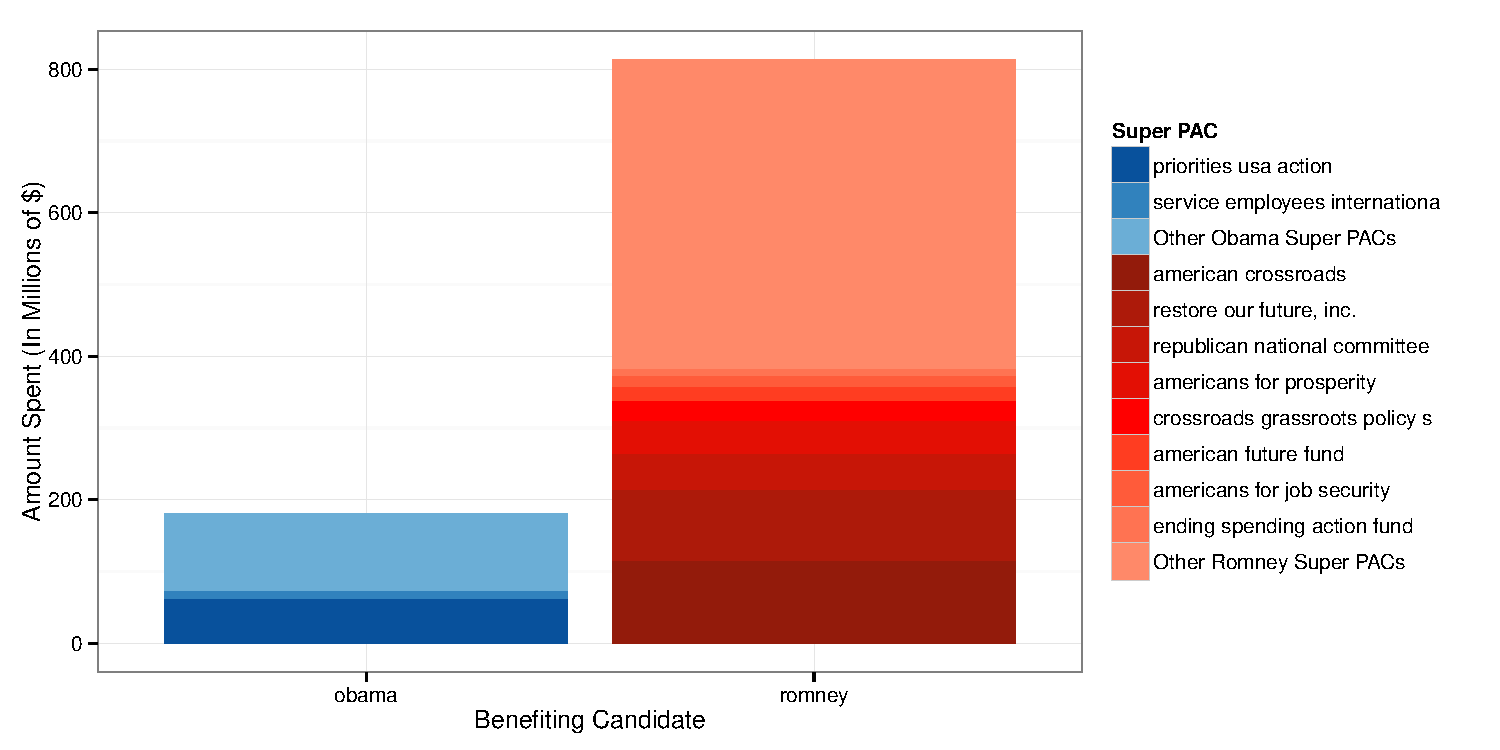
\includegraphics[width=\textwidth]{figure/PAC_plot} 

}

\caption[Spending by Super PAC, stacked by candidate]{Spending by Super PAC, stacked by candidate.\label{fig:PAC_plot}}
\end{figure}

\end{knitrout}




%\subsection{Swing State Trends}

Figure \ref{fig:type_swing_1} displays the change in polling support for both Mr. Romney and Mr. Obama over time, in 12 swing states.  Figure \ref{fig:swing_map} highlights these particular states.

\begin{knitrout}
\definecolor{shadecolor}{rgb}{0.969, 0.969, 0.969}\color{fgcolor}\begin{figure}[H]


{\centering 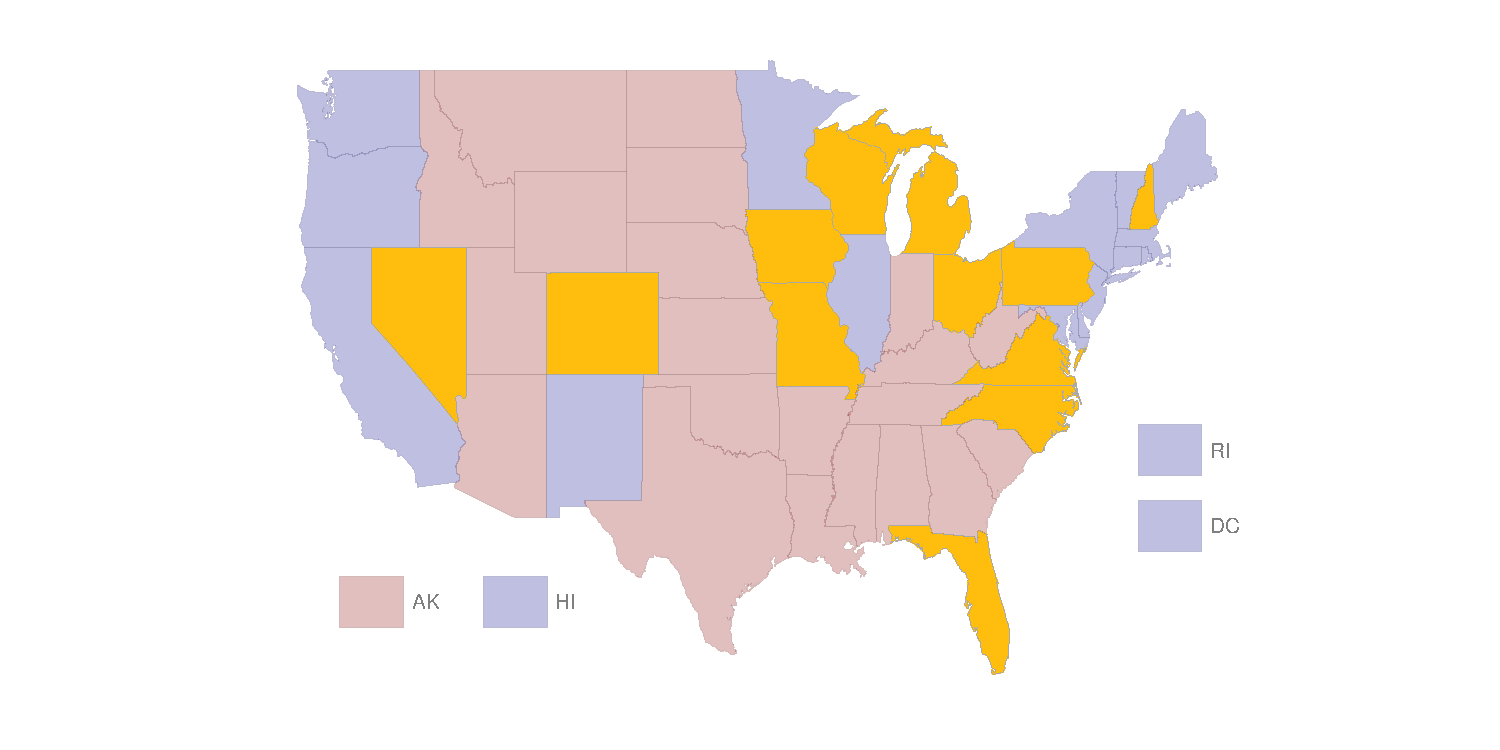
\includegraphics[width=\textwidth]{figure/swing_map} 

}

\caption[Map of United States with swing states highlighted]{Map of United States with swing states highlighted.\label{fig:swing_map}}
\end{figure}

\end{knitrout}


The data includes all polls in the NationalPolls.com database from April 25th to November 6th. Percent support for each candidate is shown for each state with a smoothed line indicating trend. There are five markers which signify major events in the campaign: the selection of Mr. Ryan as Mr. Romney's vice presidential nominee, the Republican National Convention, the Democratic National Convention, the 47\% video and the first presidential debate. 

The plots suggest that the reaction to these major campaign events was not consistent state to state. Some states, such as Wisconsin, have produced drastic changes in polling support over time (``bounces"), while others, such as North Carolina, have maintained a consistent margin of support for the two candidates.

\begin{knitrout}
\definecolor{shadecolor}{rgb}{0.969, 0.969, 0.969}\color{fgcolor}\begin{figure}[H]


{\centering 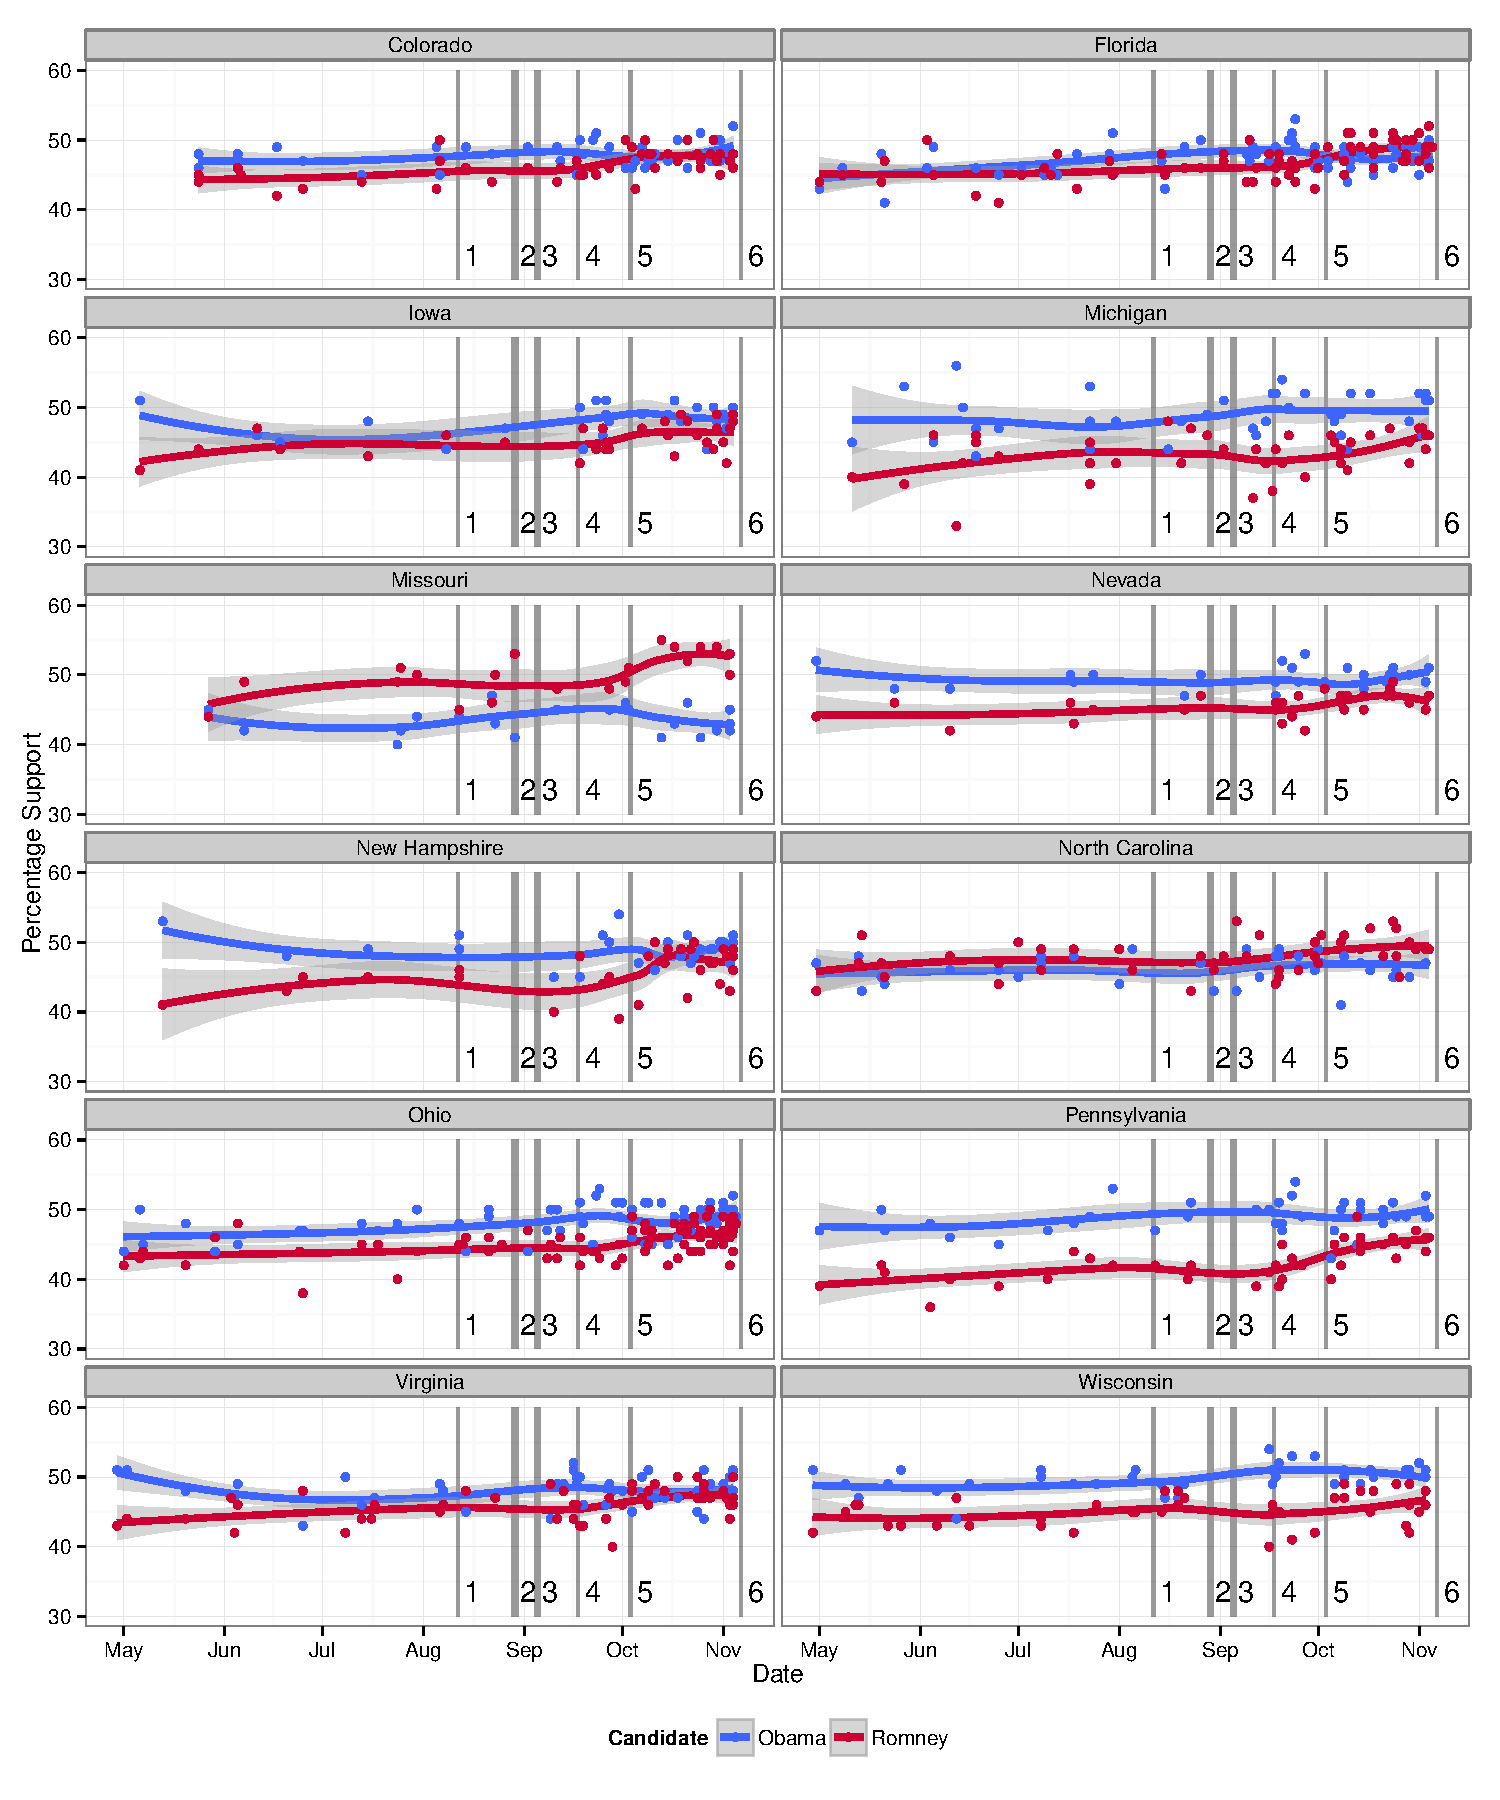
\includegraphics[width=\textwidth]{figure/type_swing_1} 

}

\caption[Polling averages for Mr]{Polling averages for Mr. Obama and Mr. Romney by swing state. Important events are indicated as follows: (1) Paul Ryan VP selection, (2) Republican National Convention, (3) Democratic National Convention, (4) 47\% video leaked, (5) first presidential debate, and (6) election day.\label{fig:type_swing_1}}
\end{figure}

\end{knitrout}



%\subsection{Spending by Week}

Figure \ref{fig:trend_plot} shows weekly spending by PACs benefiting either candidate. Looking at weekly spending by PACs benefiting Mr. Romney, we can see a sharp increase in spending that occurred during the week of July 18th. We examine at the national and swing state polls to determine if there is any noticeable effect due to these changes in spending in the weeks following.
%Similarly, there was a sharp increase in spending by Obama-supporting PACs during the week of September 9th. 

\begin{knitrout}
\definecolor{shadecolor}{rgb}{0.969, 0.969, 0.969}\color{fgcolor}\begin{figure}[H]


{\centering 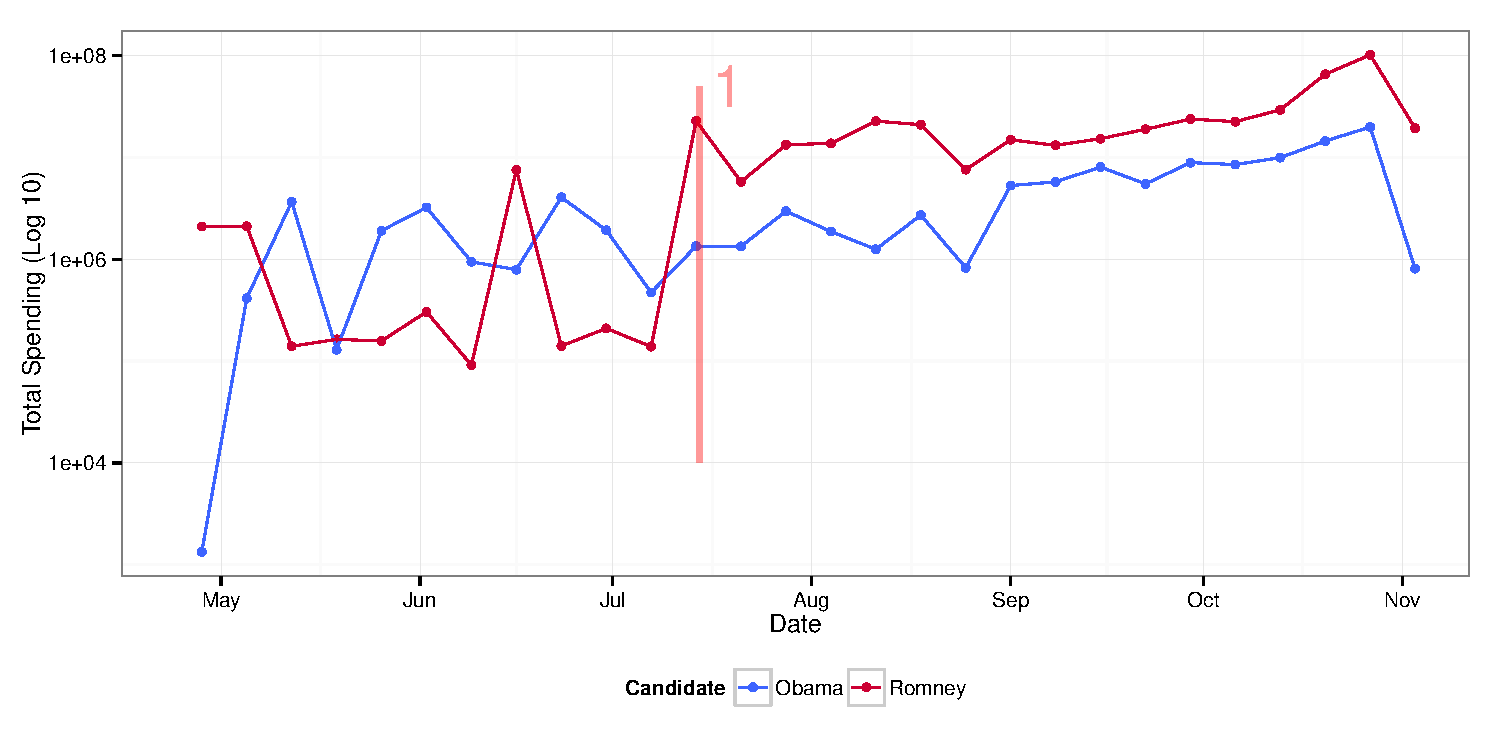
\includegraphics[width=\textwidth]{figure/trend_plot} 

}

\caption[Weekly spending by Super PACs supporting Mr]{Weekly spending by Super PACs supporting Mr. Obama and Mr. Romney. Shaded region (1) indicates a period of lower spending by Super PACs supporting Mr. Romney and unshaded region (2) indicates a period of higher spending.\label{fig:trend_plot}}
\end{figure}

\end{knitrout}


%\subsection{Effect of Spending on Polls}

Figure \ref{fig:effect_plot} shows the polling margin (Obama - Romney) over time, colored by swing states versus the national polls. It can be seen that Mr. Obama consistently maintained an advantage in swing states relative to his national numbers. A marker is placed on July 18th, corresponding to the sharp increase in spending by PACs supporting Mr. Romney. It does not seem that this spending increase had a measurable effect on the overall trend in the polls at this time.

Note that this plot utilizes exponential smoothing to show the trends in polls over time rather than a LOESS smoother, as we have used previously. When using the LOESS smoother, the future polling numbers were heavily affecting the smoothed trend line, which was undesirable. This is because the LOESS smoother takes points past and future with equal weight into account when showing the trend. However, the exponential smoothing method places importance on past points with exponentially decreasing weights as the points become further from the event, limiting the impact of future polling on the current smoothed trend. We implemented the exponential smoothing method using the \texttt{forecast} and \texttt{zoo} packages.

\begin{knitrout}
\definecolor{shadecolor}{rgb}{0.969, 0.969, 0.969}\color{fgcolor}\begin{figure}[H]


{\centering 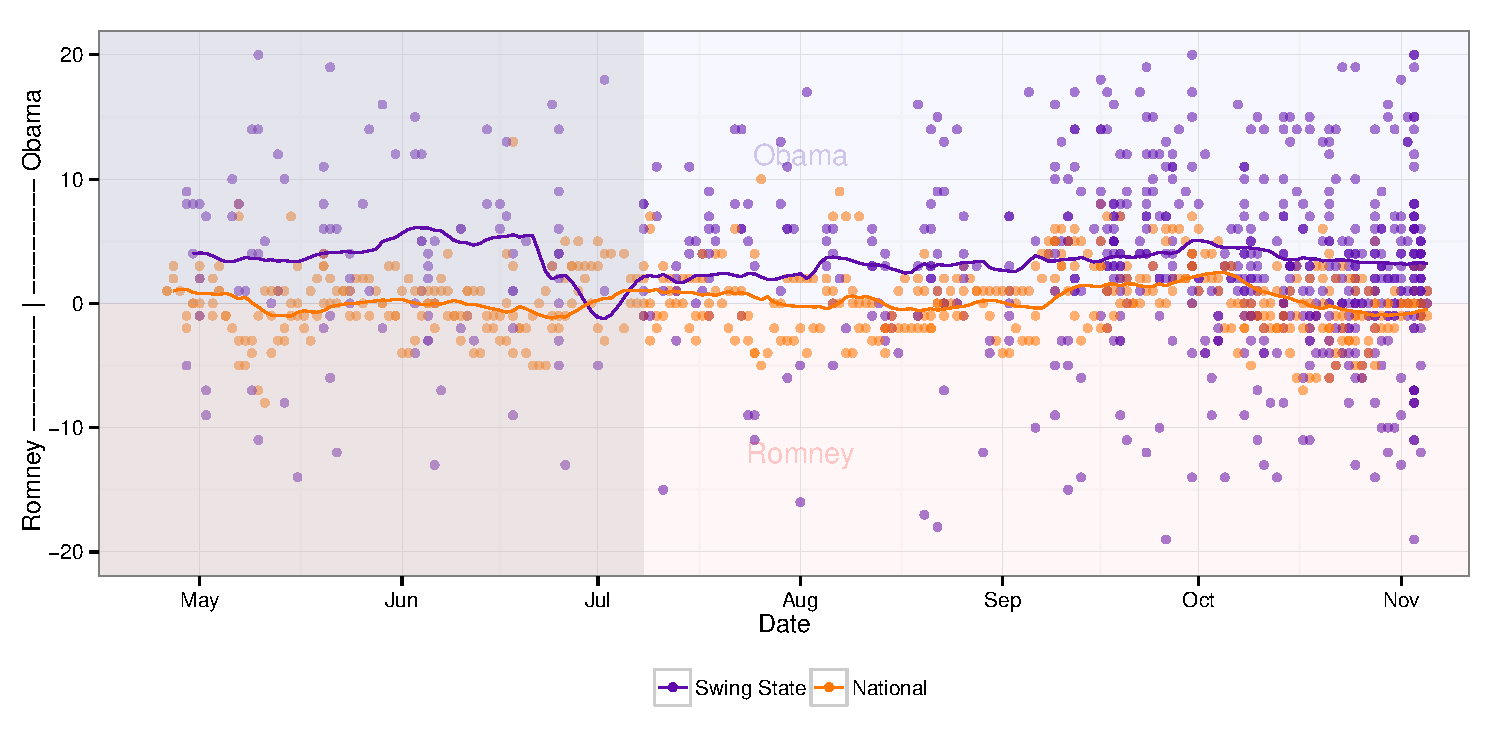
\includegraphics[width=\textwidth]{figure/effect_plot} 

}

\caption[Polling margin (Obama - Romney) over time, swing states versus national polls]{Polling margin (Obama - Romney) over time, swing states versus national polls. Shaded region indicates a period of lower spending by Super PACs supporting Mr. Romney and unshaded region indicates a period of higher spending.\label{fig:effect_plot}}
\end{figure}

\end{knitrout}


Figure \ref{fig:support_spend} compares the difference in PAC spending by week to the difference in polling between Mr. Romney and Mr. Obama with a one week lag. The points are colored by week and certain weeks are labeled to indicated important events. The goal is to see if there is a relationship between PAC spending and poll results. In PACs supporting both Mr. Obama and Mr. Romney we can see a weak positive relationship between spending and polling.

\begin{knitrout}
\definecolor{shadecolor}{rgb}{0.969, 0.969, 0.969}\color{fgcolor}\begin{figure}[H]


{\centering 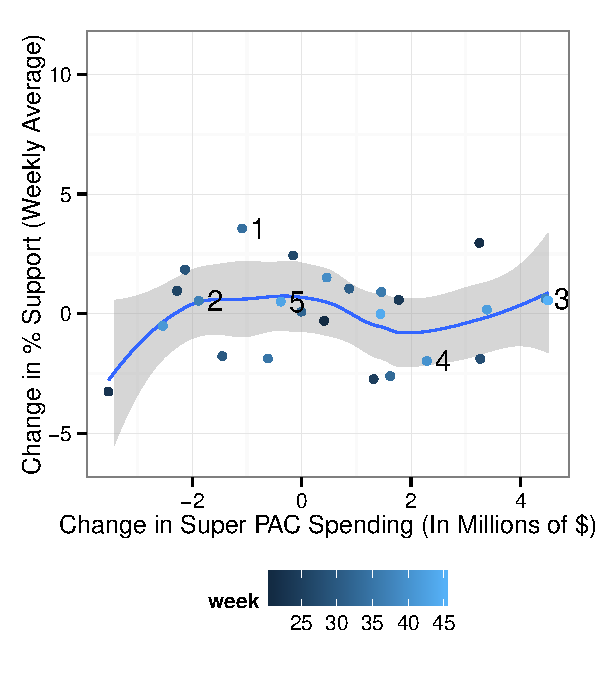
\includegraphics[width=.45\textwidth]{figure/support_spend1} 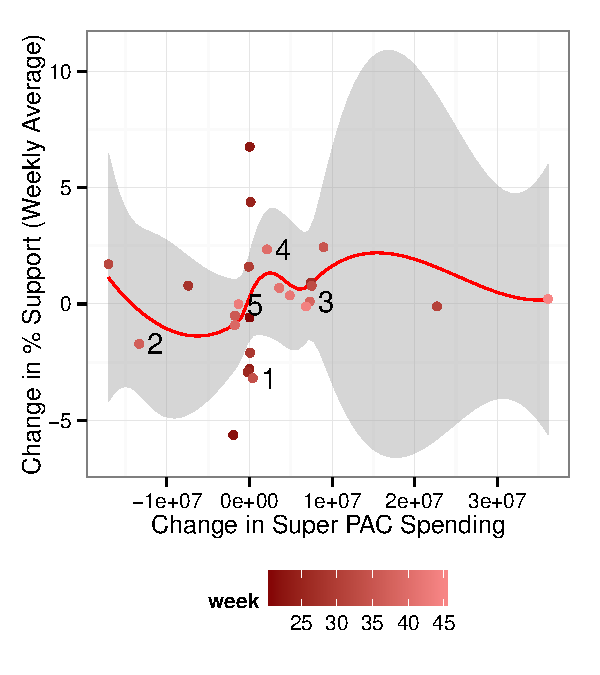
\includegraphics[width=.45\textwidth]{figure/support_spend2} 

}

\caption[Change in polling over change in spending by candidate]{Change in polling over change in spending by candidate. Important events are indicated as follows: (1) Paul Ryan VP selection, (2) Republican National Convention, (3) Democratic National Convention, (4) 47\% video leaked, and (5) first presidential debate.\label{fig:support_spend}}
\end{figure}

\end{knitrout}


\section{Conclusions/Future Work}
Ultimately, our findings suggest that while election spending itself was a very significant part of the 2012 elections, it is not clear whether the existence of Super PACs had a measurable impact on the outcome of the presidential race. Instead, the events that garnered large amounts of media coverage, such as the 47\% video and the first presidential debate, seem to have had the most noticeable effect on the polling. Furthermore, our analysis did not take into account the spending done by the candidates themselves. It may be that such spending muted the effect of Super PAC spending.

We did discover interesting spending patterns by the Super PACs. Although Super PACs supporting Mr. Romney spent significantly more over the course of the campaign, they spent less than Super PACs supporting Mr. Obama in all but one week from mid-May until mid-July. This is in spite of the fact that the Republican primary was effectively finished by late-April. It will be interesting to see whether large spending begins earlier in the election season in future presidential campaigns.

Our analysis also makes clear that Mr. Obama's polling held up more strongly in the swing states than in the national polling throughout the campaign. This advantage was evident in the election results, as well. According to the current certified vote tally as of December 4th\footnote{\href{https://docs.google.com/spreadsheet/lv?key=0AjYj9mXElO_QdHpla01oWE1jOFZRbnhJZkZpVFNKeVE&toomany=true}{Wasserman's 2012 National Popular Vote Tracker}}, Mr. Obama won the overall popular vote by 3.6\%. But he won Colorado, the state that put him over the 270 electoral votes needed for victory, by 5.4\%. This suggests that Mr. Obama could have lost the popular vote by nearly 2\% and still have been elected president of the United States.

Another interesting feature of our analysis is the non-uniform effect of the major events in the campaign on the polling. For instance, Mr. Ryan's selection as Mr. Romney's Vice Presidential nominee seemed to have no effect on the polls in his home state of Wisconsin. However, in Missouri, Mr. Ryan's selection coincided with a noticable increase in support for Mr. Romney. A similar trend can be seen with the release of the 47\% video. Following the release, Mr. Obama's support seemed to expand in Ohio. But in Colorado, and opposite effect is observed. The only event which seemed to produce a rather uniform change in the polls was the first presidential debate, where Mr. Romney gained support in nearly all swing states.

An extension of this project should take into account spending done by the candidates themselves, in addition to independent expenditures. This would allow for a more informed look at the relative spending difference, and how it may or may not correlate with changes in the polling averages. Another area of exploration would be the purpose field of the independent expenditures data set. Our analysis attempted to categorize spending entries into broad categories, but many of the entries in the database have more specific information. For instance, an ad buy may list the name of the ad, as well as the state the ad is running in. It may also be possible to incorporate another data source in order to link the expenditure entries with ad buys in particular states.


\end{document}
